\chapter{SYSTEM DESIGN}

The architecture of the air mouse glove, illustrated in Figure \ref{fig:system-design}, is structured around three functional layers: the sensor input layer, the processing and communication core, and the host device interface. Together, these layers form a complete wireless human-computer interaction system embedded within a wearable glove form factor.

\begin{figure}[hb]
    \centering
    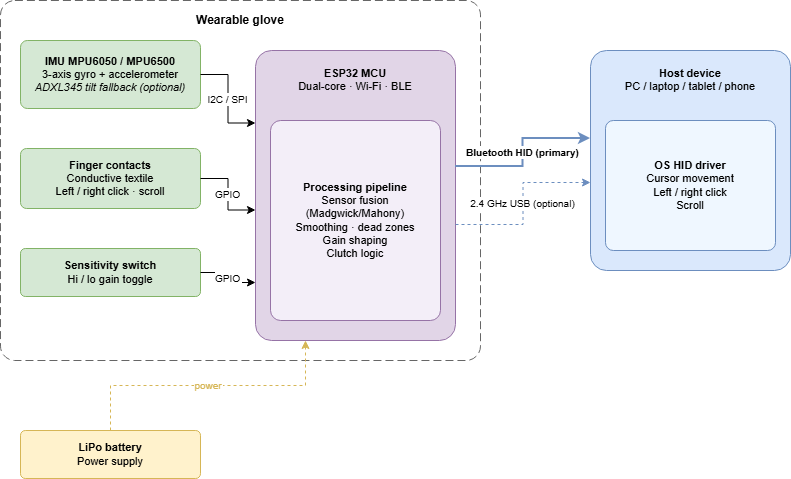
\includegraphics[width=0.9\textwidth]{img/architectural_final.drawio.png}
    \caption{System Architecture}
    \label{fig:system-design}
\end{figure}

\section*{Sensor Input Layer}

The primary motion sensing component is the \textbf{MPU-6050} (or its lower-cost variant, the MPU-6500), a six-axis Inertial Measurement Unit (IMU) that combines a 3-axis gyroscope and a 3-axis accelerometer on a single chip. The gyroscope measures angular velocity across the roll, pitch, and yaw axes, while the accelerometer captures linear acceleration and gravitational orientation. Together, these two data streams allow the system to reconstruct the full spatial orientation of the user's hand in real time. For scenarios requiring enhanced tilt accuracy or redundancy, an \textbf{ADXL345} accelerometer can be incorporated as an optional fallback device. Both the MPU-6050 and the ADXL345 communicate with the ESP32 microcontroller over the \textbf{I\textsuperscript{2}C or SPI} serial interfaces, which allow multiple devices to share the same communication bus with minimal wiring overhead.

User input beyond motion is handled by two additional components connected via \textbf{GPIO} pins on the ESP32. The \textbf{finger contact sensors}, implemented using conductive textile integrated into the glove's fingertips, detect discrete touch events and are mapped to left click, right click, and scroll actions, directly mirroring the button layout of a conventional mouse. A dedicated \textbf{sensitivity switch} provides a hardware-level \textit{hi/lo gain toggle}, enabling the user to switch between a high-sensitivity mode (suitable for fine cursor control) and a low-sensitivity mode (better suited for broad movements across large displays), without requiring any software interaction.

\section*{Processing and Communication Core}

The central processing unit of the system is the \textbf{ESP32 microcontroller}, a dual-core, 32-bit system-on-chip that integrates both \textbf{Wi-Fi} and \textbf{Bluetooth Low Energy (BLE)} radios. Its dual-core architecture allows sensor acquisition and data transmission to run concurrently without blocking each other, which is critical for maintaining low-latency cursor response.

Raw IMU data is passed through a multi-stage \textbf{processing pipeline} before being transmitted. The first stage applies a \textbf{sensor fusion algorithm}, specifically either the \textit{Madgwick} or \textit{Mahony} filter, which mathematically combines gyroscope and accelerometer readings to produce a stable quaternion-based orientation estimate. These complementary filters are computationally efficient and well-suited for embedded systems, correcting gyroscope drift over time using accelerometer gravity references. The fused orientation data is then processed through several additional stages: \textbf{smoothing filters} reduce high-frequency noise caused by natural hand tremors; \textbf{dead zones} suppress very small, unintentional movements below a configurable threshold so the cursor remains stationary when the hand is at rest; \textbf{gain shaping} applies a non-linear transfer function to map hand movement magnitude to cursor displacement speed, allowing slow movements to produce fine precision while fast movements yield rapid cursor travel; and \textbf{clutch logic} provides a mechanism to temporarily suspend cursor movement, enabling the user to reposition their hand without unintended cursor drift.

\section*{Host Device Interface}

Once processed, the orientation and button data is transmitted to the host device primarily via \textbf{Bluetooth HID} (Human Interface Device profile). This standard protocol allows the glove to present itself to any host operating system as a native wireless pointing device, requiring no proprietary drivers or software installation on PCs, laptops, tablets, or smartphones. As an optional alternative, a \textbf{2.4 GHz USB dongle} connection is also supported, which can offer lower latency in environments with Bluetooth interference.

On the host side, the operating system's built-in \textbf{HID driver} interprets the incoming data packets and translates them directly into standard \textbf{cursor movement}, \textbf{left/right click}, and \textbf{scroll} events, identical in behavior to those generated by a conventional mouse.

\section*{Power Supply}

The entire system is powered by a \textbf{LiPo} (Lithium Polymer) battery integrated into the glove. LiPo cells are well suited for this application due to their high energy density, lightweight form factor, and flat, flexible packaging that conforms naturally to wearable enclosures. The battery supplies power to both the ESP32 and all connected sensors through an onboard power regulation circuit.

\section{FR Air Glove --- UML and Architecture Diagrams}

\subsection{Overview}

Based on the analyzed implementation, \textbf{FR Air Glove} is an ESP32-based wearable BLE HID mouse. The system reads hand motion from an MPU6050 IMU and capacitive touch input from ESP32 touch pads. This input is processed by driver modules, service modules, FreeRTOS tasks, and finally converted into BLE HID mouse reports sent to a paired host device.

The diagrams in this section describe the project from different viewpoints: user functionality, high-level architecture, runtime activities, and sequence interactions between the main software modules. Each diagram is based on the real code structure and uses the actual module or function names where necessary.

\subsection{UML Use Case Diagram}

\begin{figure}[H]
    \centering
   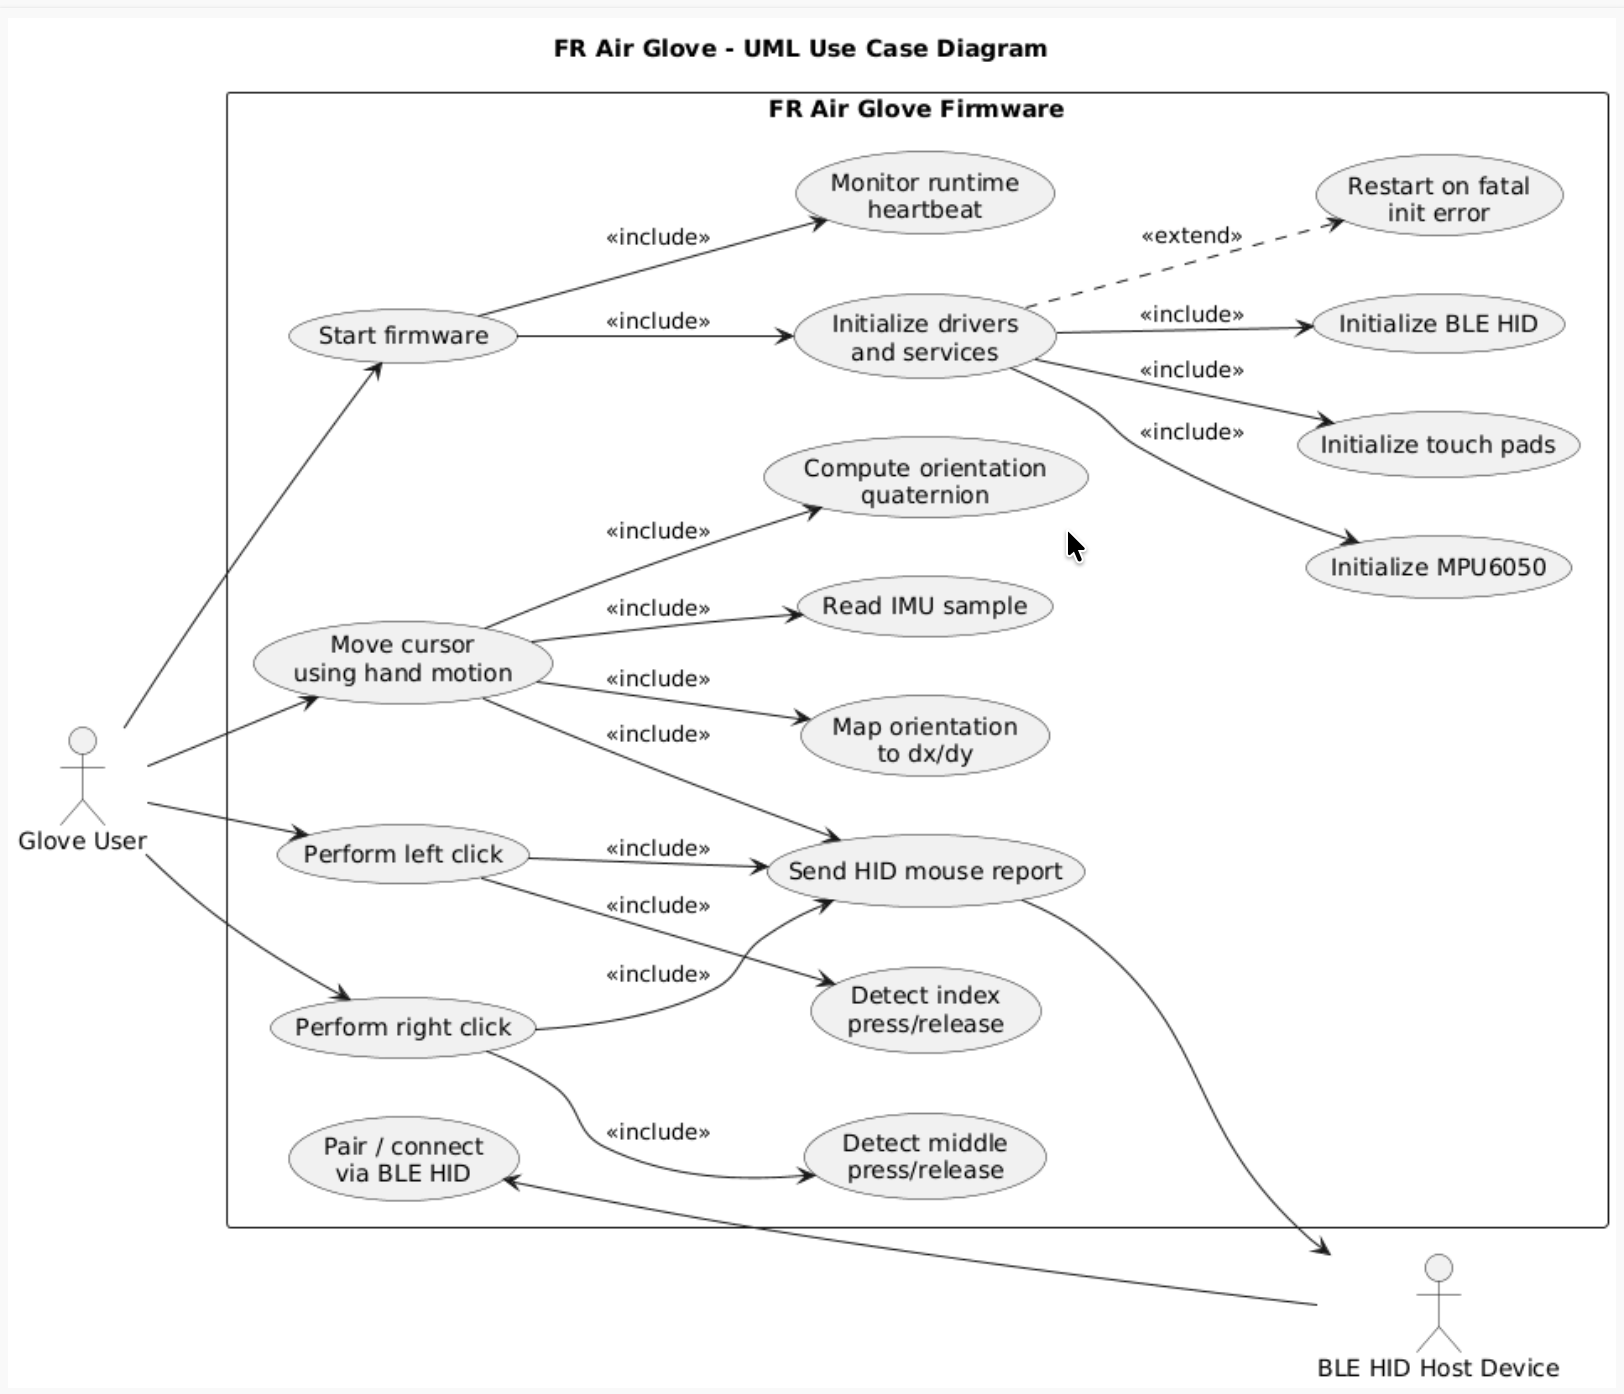
\includegraphics[width=0.5\textwidth]{img/use-case.png}
    \caption{FR Air Glove UML Use Case Diagram}
    \label{fig:fr-air-glove-use-case}
\end{figure}

The use case diagram presents the FR Air Glove system from the external user perspective. The main actor is the \textbf{Glove User}, who interacts with the device by powering it on, moving the hand, and touching specific capacitive pads. These actions are translated into mouse functions such as cursor movement, left click, and right click. The second actor is the \textbf{BLE HID Host Device}, which represents a computer, tablet, or phone that receives the HID mouse input through Bluetooth.

The system boundary represents the firmware running on the ESP32. Inside this boundary are the main functions supported by the system: starting the firmware, initializing drivers and services, pairing through BLE HID, reading IMU data, calculating orientation, mapping motion to cursor movement, detecting touch press/release actions, and sending HID mouse reports.

This diagram is useful because it gives a general overview of what the system does before explaining how the internal modules work. It also separates user-level functionality from implementation details.

Code support examples:
\begin{itemize}
    \item Firmware startup begins in \texttt{setup()}, which calls \texttt{app\_controller\_start()}.
    \item Initialization is supported by \texttt{dd\_mpu6050\_init()}, \texttt{dd\_touch\_init()}, and \texttt{dd\_ble\_hid\_init()}.
    \item Cursor movement is supported by \texttt{dd\_mpu6050\_read()}, \texttt{srv\_fusion\_update()}, and \texttt{srv\_motion\_update()}.
    \item Touch clicking is supported by \texttt{srv\_input\_process()} and the button mapping inside the application task.
\end{itemize}

\subsection{High-Level Architecture Diagram}

\begin{figure}[H]
    \centering
    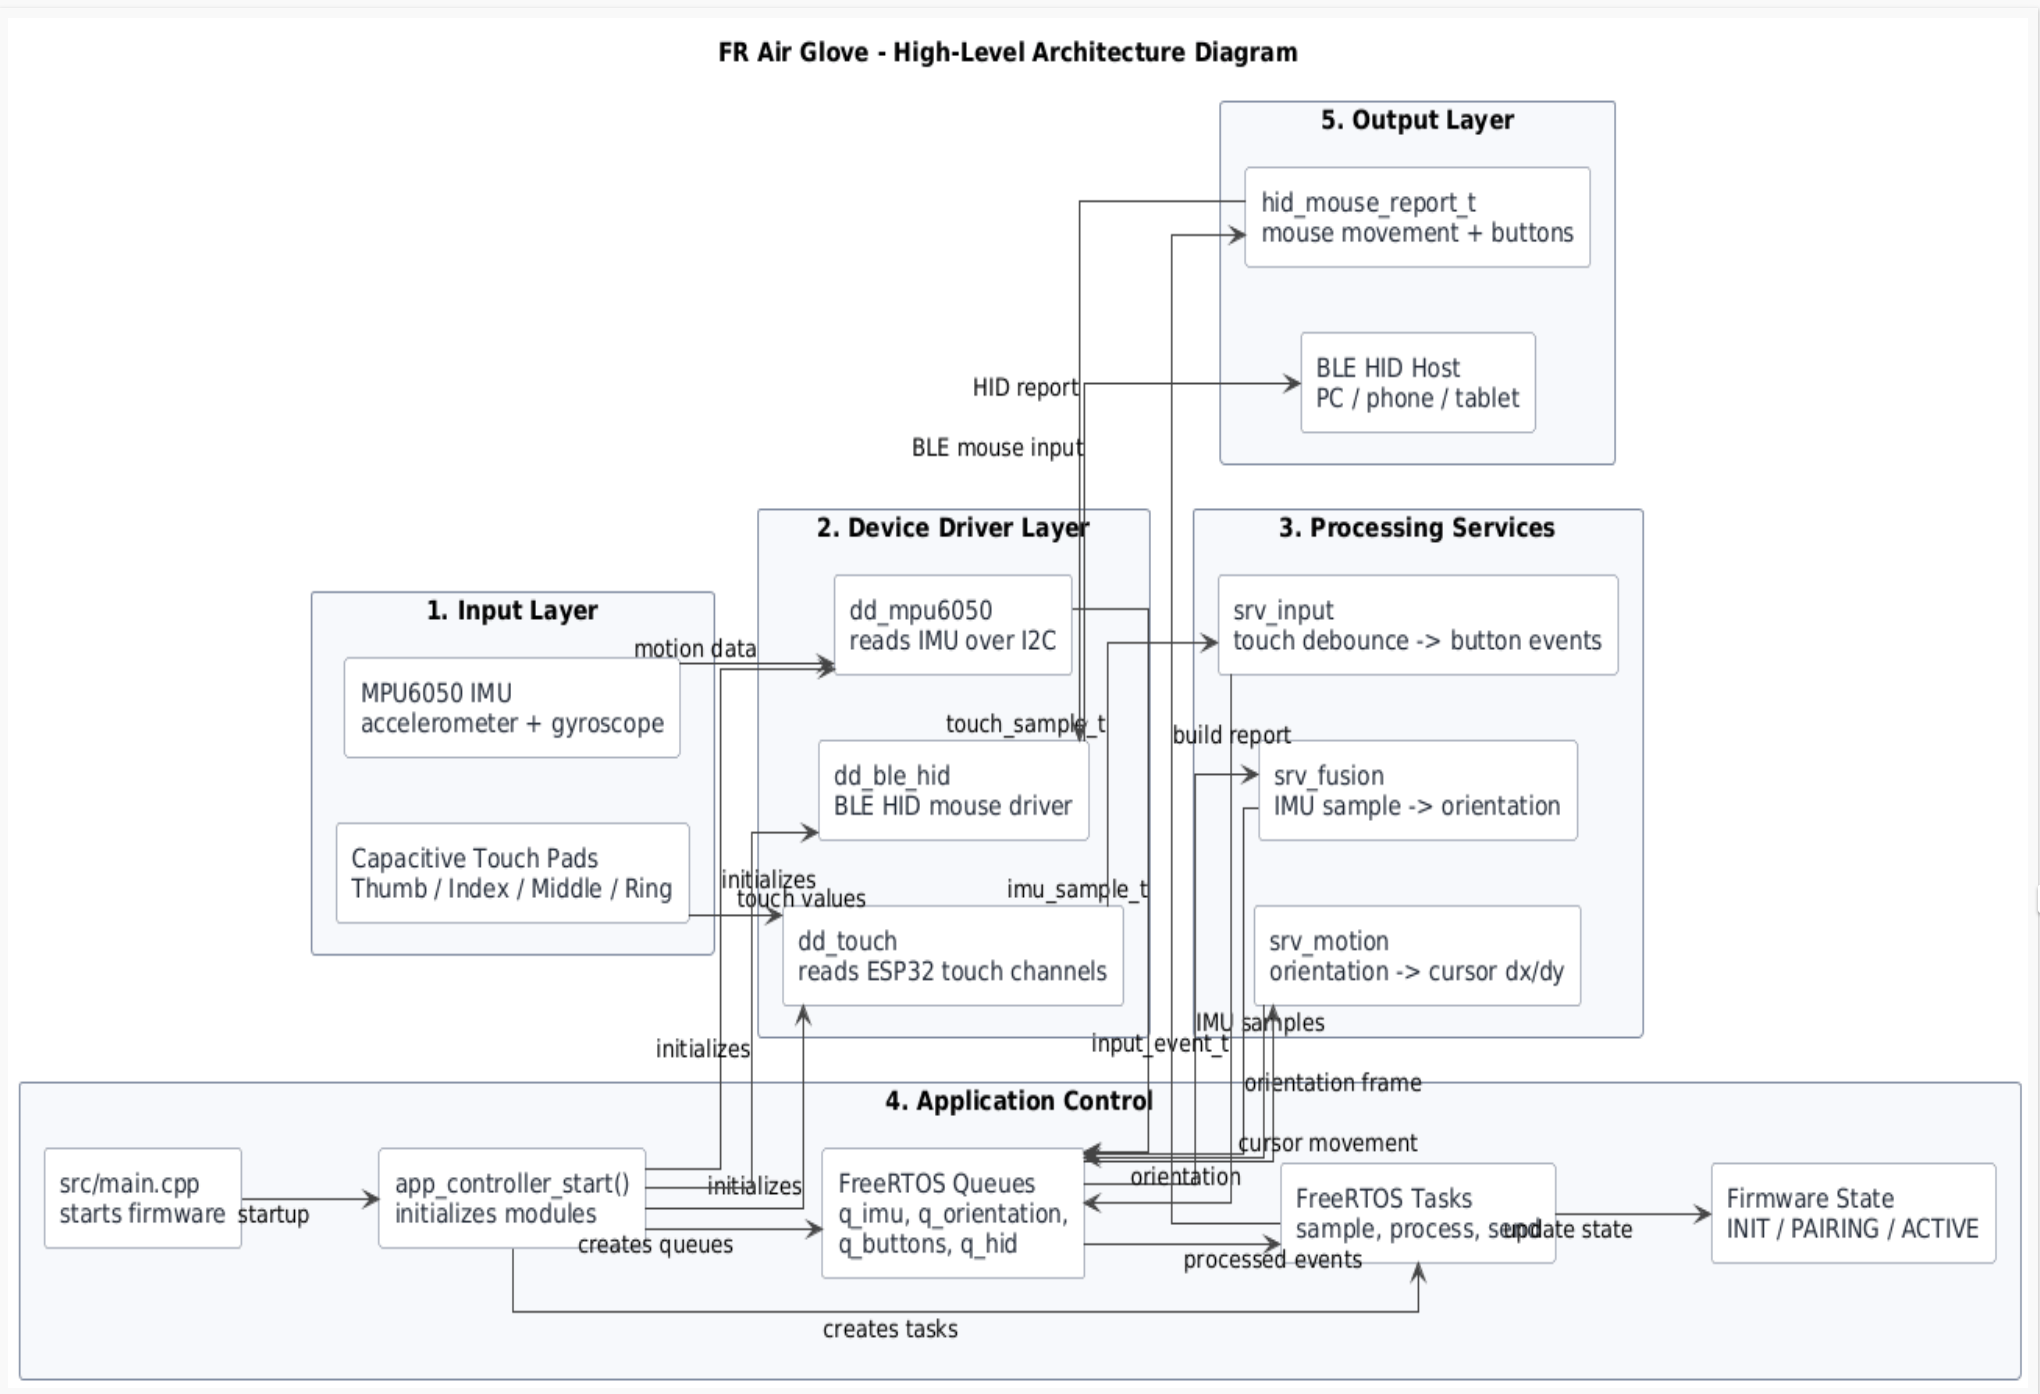
\includegraphics[width=0.8\textwidth]{img/h-l.png}
    \caption{FR Air Glove High-Level Architecture Diagram}
    \label{fig:fr-air-glove-high-level-architecture}
\end{figure}

The high-level architecture diagram shows the system as a set of logical layers. The first layer is the input layer, where the MPU6050 IMU provides movement data and the capacitive touch pads provide button input. The second layer is the device driver layer, which contains hardware-specific modules responsible for reading sensors and handling BLE HID communication.

The processing services layer transforms raw data into meaningful control data. The fusion service estimates glove orientation, the motion service converts orientation changes into cursor movement, and the input service filters touch readings into stable button events. The application control layer coordinates the system using FreeRTOS tasks and queues. Finally, the output layer contains the HID report structure and the external BLE HID host.

This architecture is important because it shows that the firmware is modular. Hardware access, processing logic, runtime control, and communication are separated into different responsibilities. This makes the project easier to understand, test, and extend.

Code support examples:
\begin{itemize}
    \item The driver layer is represented by \texttt{dd\_mpu6050}, \texttt{dd\_touch}, and \texttt{dd\_ble\_hid}.
    \item The processing layer is represented by \texttt{srv\_fusion}, \texttt{srv\_motion}, and \texttt{srv\_input}.
    \item The application layer is started through \texttt{app\_controller\_start()}.
    \item The final output is represented by \texttt{hid\_mouse\_report\_t} and sent using \texttt{dd\_ble\_hid\_send()}.
\end{itemize}

\subsection{Activity Diagrams}

The main activity diagram was divided into four smaller diagrams because the firmware contains several parallel FreeRTOS-based behaviours. Splitting the activity model makes each process easier to understand and avoids creating one large unreadable diagram.

\subsubsection{System Initialization Activity}

\begin{figure}[H]
    \centering
    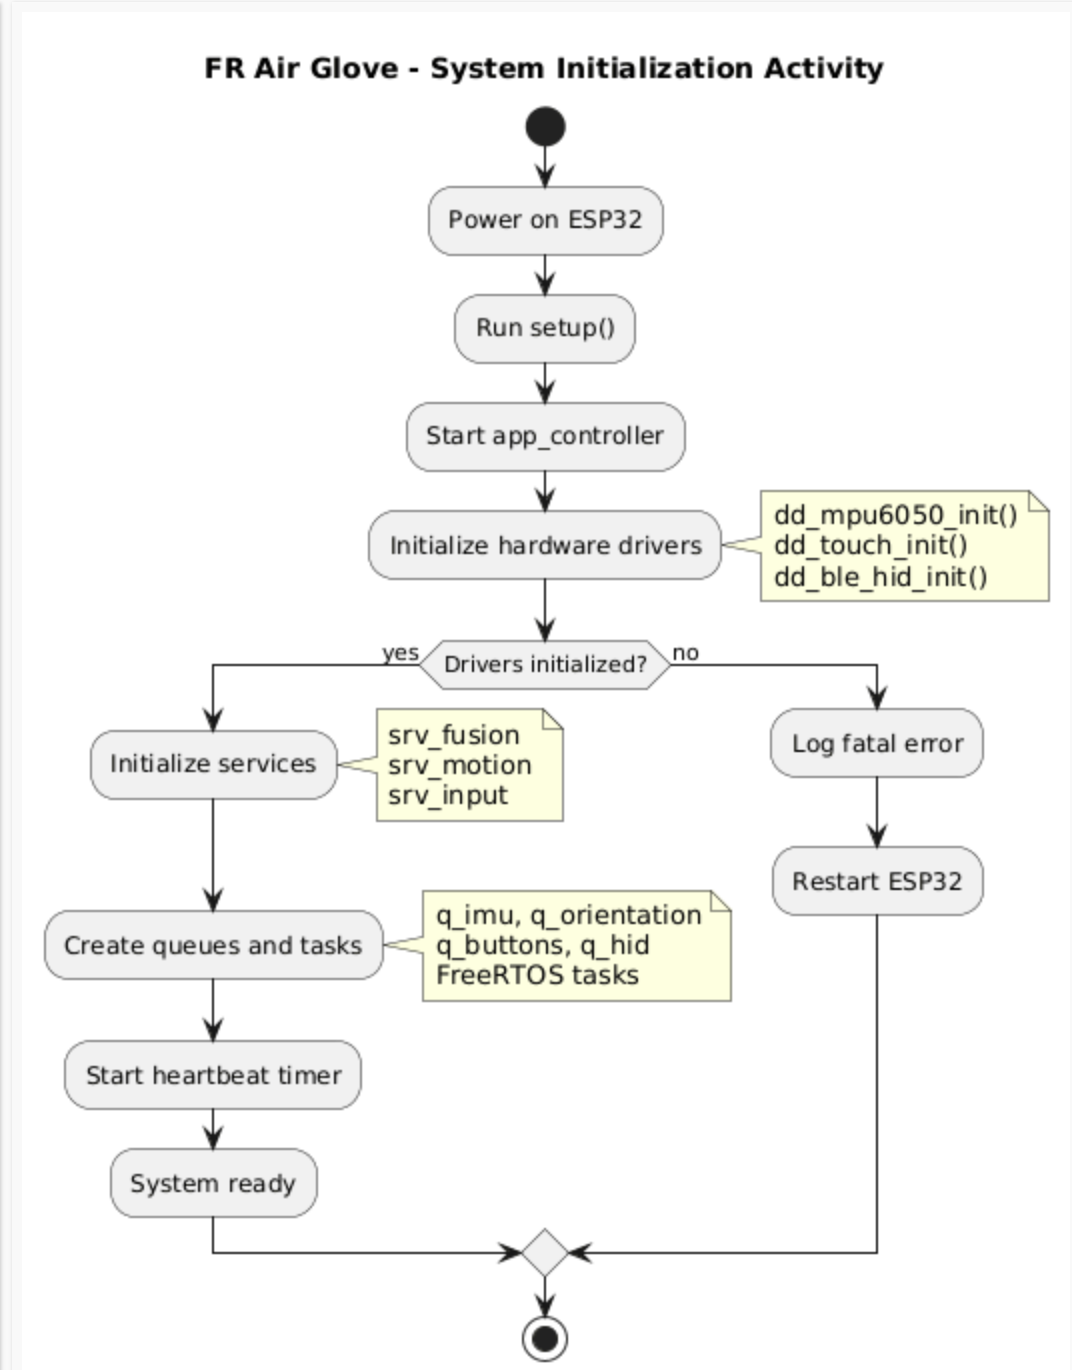
\includegraphics[width=0.5\textwidth]{img/a1.png}
    \caption{FR Air Glove System Initialization Activity Diagram}
    \label{fig:fr-air-glove-activity-initialization}
\end{figure}

The system initialization activity diagram describes how the firmware starts after the ESP32 is powered on. The process begins with the Arduino \texttt{setup()} function, which starts the application controller. The controller initializes the required hardware drivers, including the MPU6050 driver, the touch driver, and the BLE HID driver.

If driver initialization succeeds, the firmware continues by initializing the processing services. These services are responsible for sensor fusion, motion calculation, and touch input filtering. After that, the application creates FreeRTOS queues and tasks. The queues are used to transfer IMU samples, orientation data, button events, and HID reports between tasks. Finally, the heartbeat timer is started and the system becomes ready for runtime operation.

If initialization fails, the firmware follows an error path. It logs a fatal error and restarts the ESP32. This is important in embedded systems because the device should not continue running when essential hardware or communication modules are not available.

Code support examples:
\begin{itemize}
    \item Startup begins in \texttt{setup()} and continues with \texttt{app\_controller\_start()}.
    \item Hardware initialization uses \texttt{dd\_mpu6050\_init()}, \texttt{dd\_touch\_init()}, and \texttt{dd\_ble\_hid\_init()}.
    \item Service initialization uses \texttt{srv\_fusion\_init()}, \texttt{srv\_motion\_init()}, and \texttt{srv\_input\_init()}.
    \item Fatal initialization errors are handled by restarting the ESP32.
\end{itemize}

\subsubsection{IMU Motion Processing Activity}

\begin{figure}[H]
    \centering
    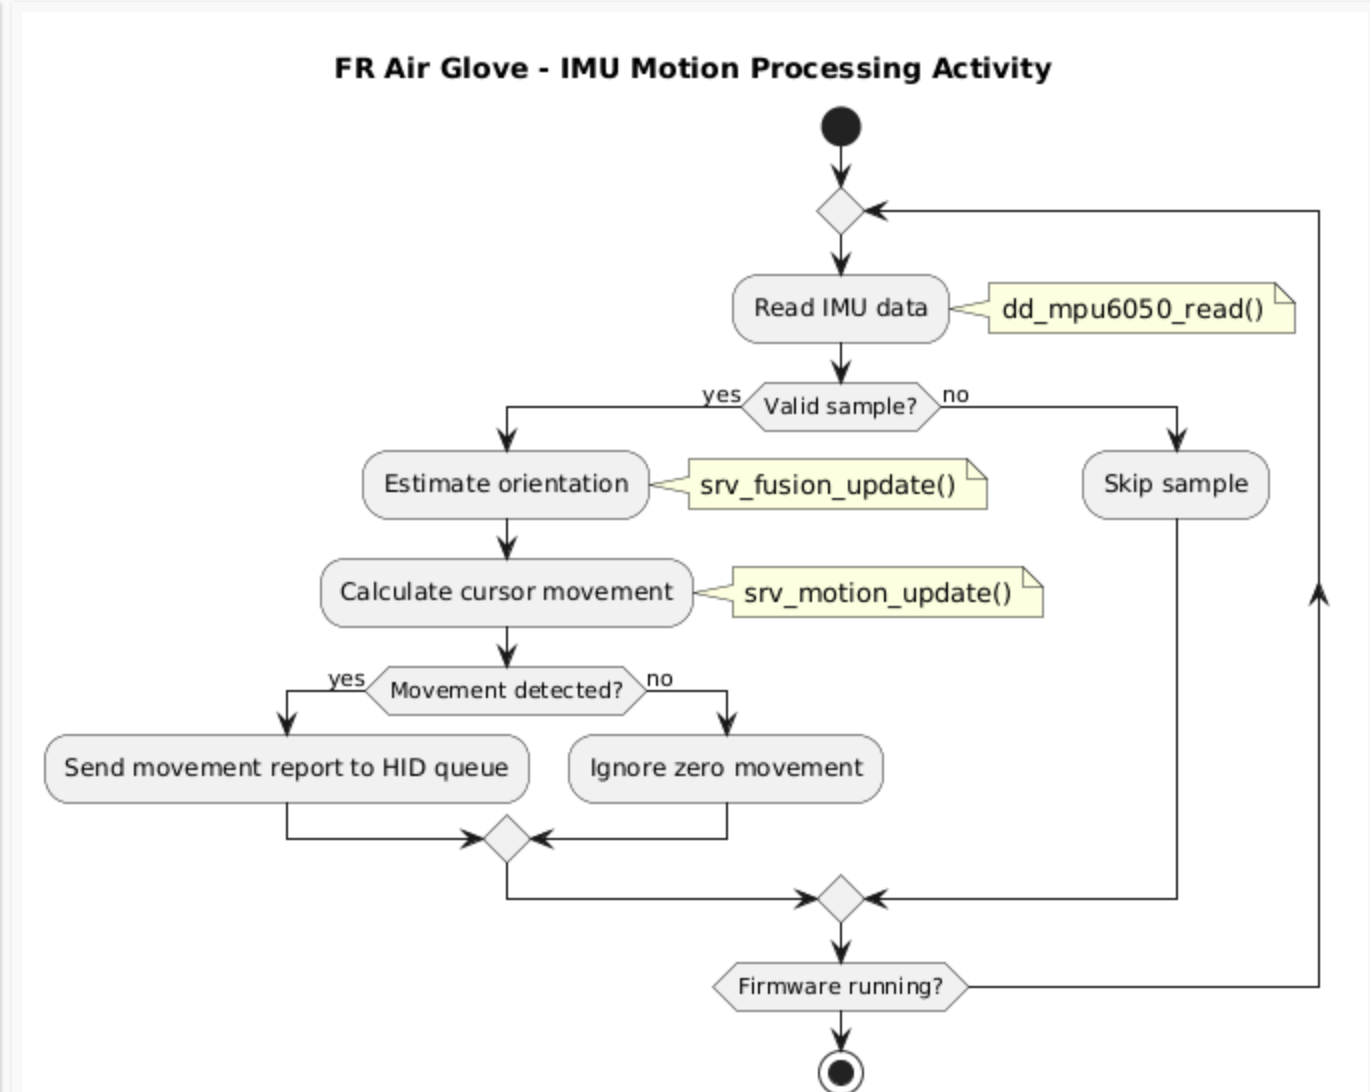
\includegraphics[width=0.5\textwidth]{img/a2.png}
    \caption{FR Air Glove IMU Motion Processing Activity Diagram}
    \label{fig:fr-air-glove-activity-imu}
\end{figure}

The IMU motion processing activity diagram explains how hand movement becomes cursor movement. The process starts by reading data from the MPU6050 IMU. If the sample is valid, the system estimates the glove orientation using the sensor fusion service. Then the motion service calculates cursor movement values from the orientation changes.

The decision point ``Movement detected?'' prevents unnecessary HID reports from being produced when there is no meaningful cursor movement. If movement is detected, a movement report is sent to the HID queue. If no movement is detected, the sample is ignored. If the IMU sample is invalid, the firmware skips the current sample and continues running.

This diagram is useful because it shows the transformation from physical hand motion to mouse cursor movement. It also shows that the firmware does not directly send every raw sensor value to the host. Instead, the data is filtered and converted into a proper HID mouse movement report.

Code support examples:
\begin{itemize}
    \item IMU data is read using \texttt{dd\_mpu6050\_read()}.
    \item Orientation estimation is performed by \texttt{srv\_fusion\_update()}.
    \item Cursor movement is calculated by \texttt{srv\_motion\_update()}.
    \item Movement results are sent as HID reports through the HID queue.
\end{itemize}

\subsubsection{Touch Button Processing Activity}

\begin{figure}[H]
    \centering
    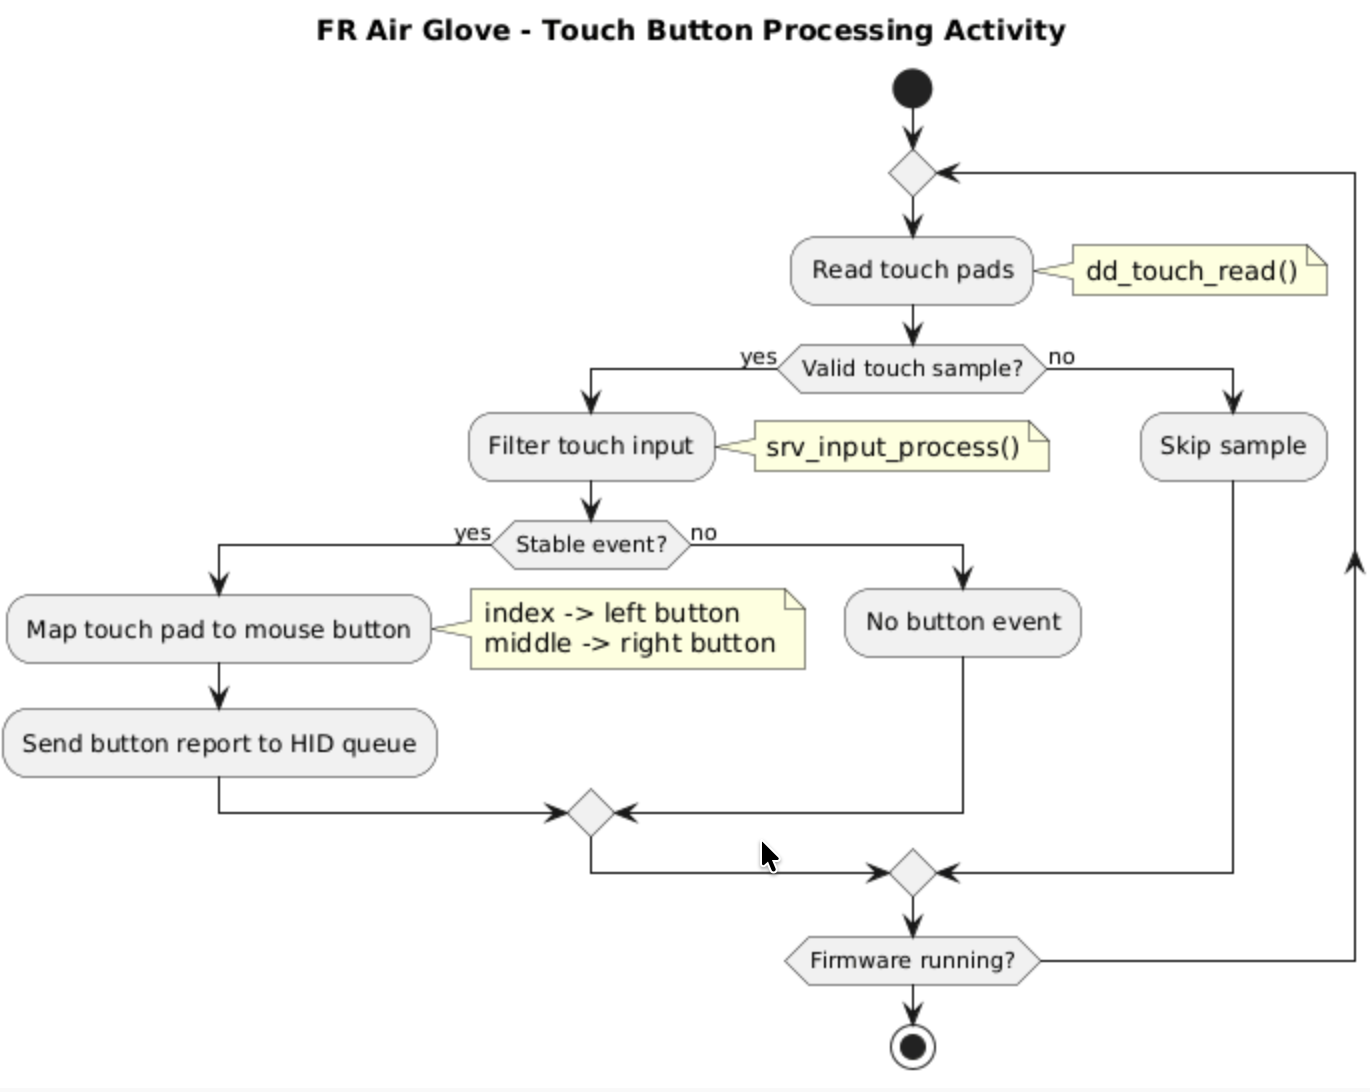
\includegraphics[width=0.5\textwidth]{img/a3.png}
    \caption{FR Air Glove Touch Button Processing Activity Diagram}
    \label{fig:fr-air-glove-activity-touch}
\end{figure}

The touch button processing activity diagram describes how capacitive touch input is converted into mouse button actions. The firmware first reads the touch pads. If the sample is valid, it is passed to the input service, which filters the data and checks whether a stable press or release event occurred.

This filtering step is necessary because capacitive touch values can be noisy. The system should not generate clicks from short glitches or unstable readings. Only stable touch events are mapped to mouse buttons. According to the implemented logic, the index pad is mapped to the left mouse button and the middle pad is mapped to the right mouse button. After mapping, a button report is sent to the HID queue.

If no stable event exists, no button event is produced. If the touch sample is invalid, the firmware skips it and continues running. This activity diagram is useful because it shows how the firmware protects the system from accidental or noisy clicks.

Code support examples:
\begin{itemize}
    \item Touch pads are read using \texttt{dd\_touch\_read()}.
    \item Touch filtering and debounce logic are handled by \texttt{srv\_input\_process()}.
    \item The index touch pad is mapped to the left mouse button.
    \item The middle touch pad is mapped to the right mouse button.
\end{itemize}

\subsubsection{BLE HID Output Activity}

\begin{figure}[H]
    \centering
    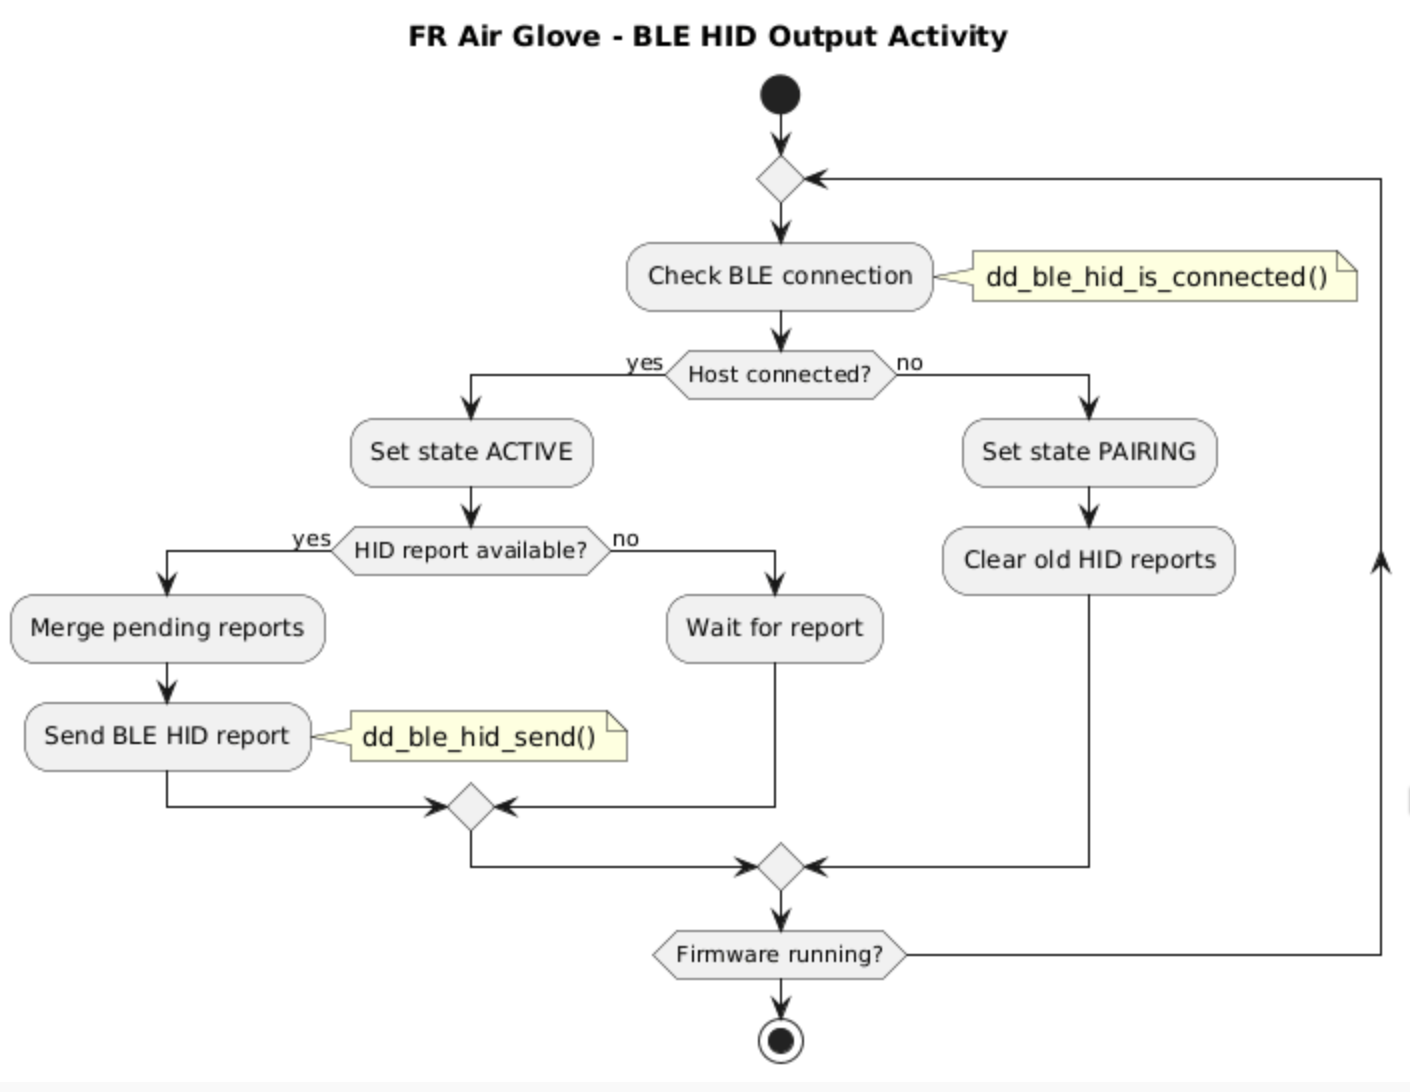
\includegraphics[width=0.5\textwidth]{img/a4.png}
    \caption{FR Air Glove BLE HID Output Activity Diagram}
    \label{fig:fr-air-glove-activity-ble}
\end{figure}

The BLE HID output activity diagram shows how prepared HID reports are sent to the external host. The firmware first checks whether a BLE HID host is connected. If the host is connected, the firmware enters the active state and checks whether a HID report is available. When a report is available, pending reports may be merged, and the final BLE HID report is sent.

If no HID report is available, the firmware waits for the next report. If the host is not connected, the firmware switches to pairing state and clears old HID reports. Clearing old reports is important because movement or click data generated before connection should not be sent later as stale input.

This diagram is useful because it shows that BLE output is controlled by connection state. The glove does not blindly send reports; it first verifies that a host is connected and then sends only valid prepared HID data.

Code support examples:
\begin{itemize}
    \item BLE connection state is checked with \texttt{dd\_ble\_hid\_is\_connected()}.
    \item The active and pairing states correspond to the firmware state logic.
    \item HID reports are represented by \texttt{hid\_mouse\_report\_t}.
    \item BLE transmission is performed using \texttt{dd\_ble\_hid\_send()}.
\end{itemize}

\subsection{Sequence Diagrams}

The sequence diagrams describe interactions between modules over time. They were divided into four smaller diagrams: firmware startup, motion-to-cursor processing, touch-to-button processing, and BLE HID transmission.

\subsubsection{Firmware Startup Sequence}

\begin{figure}[H]
    \centering
    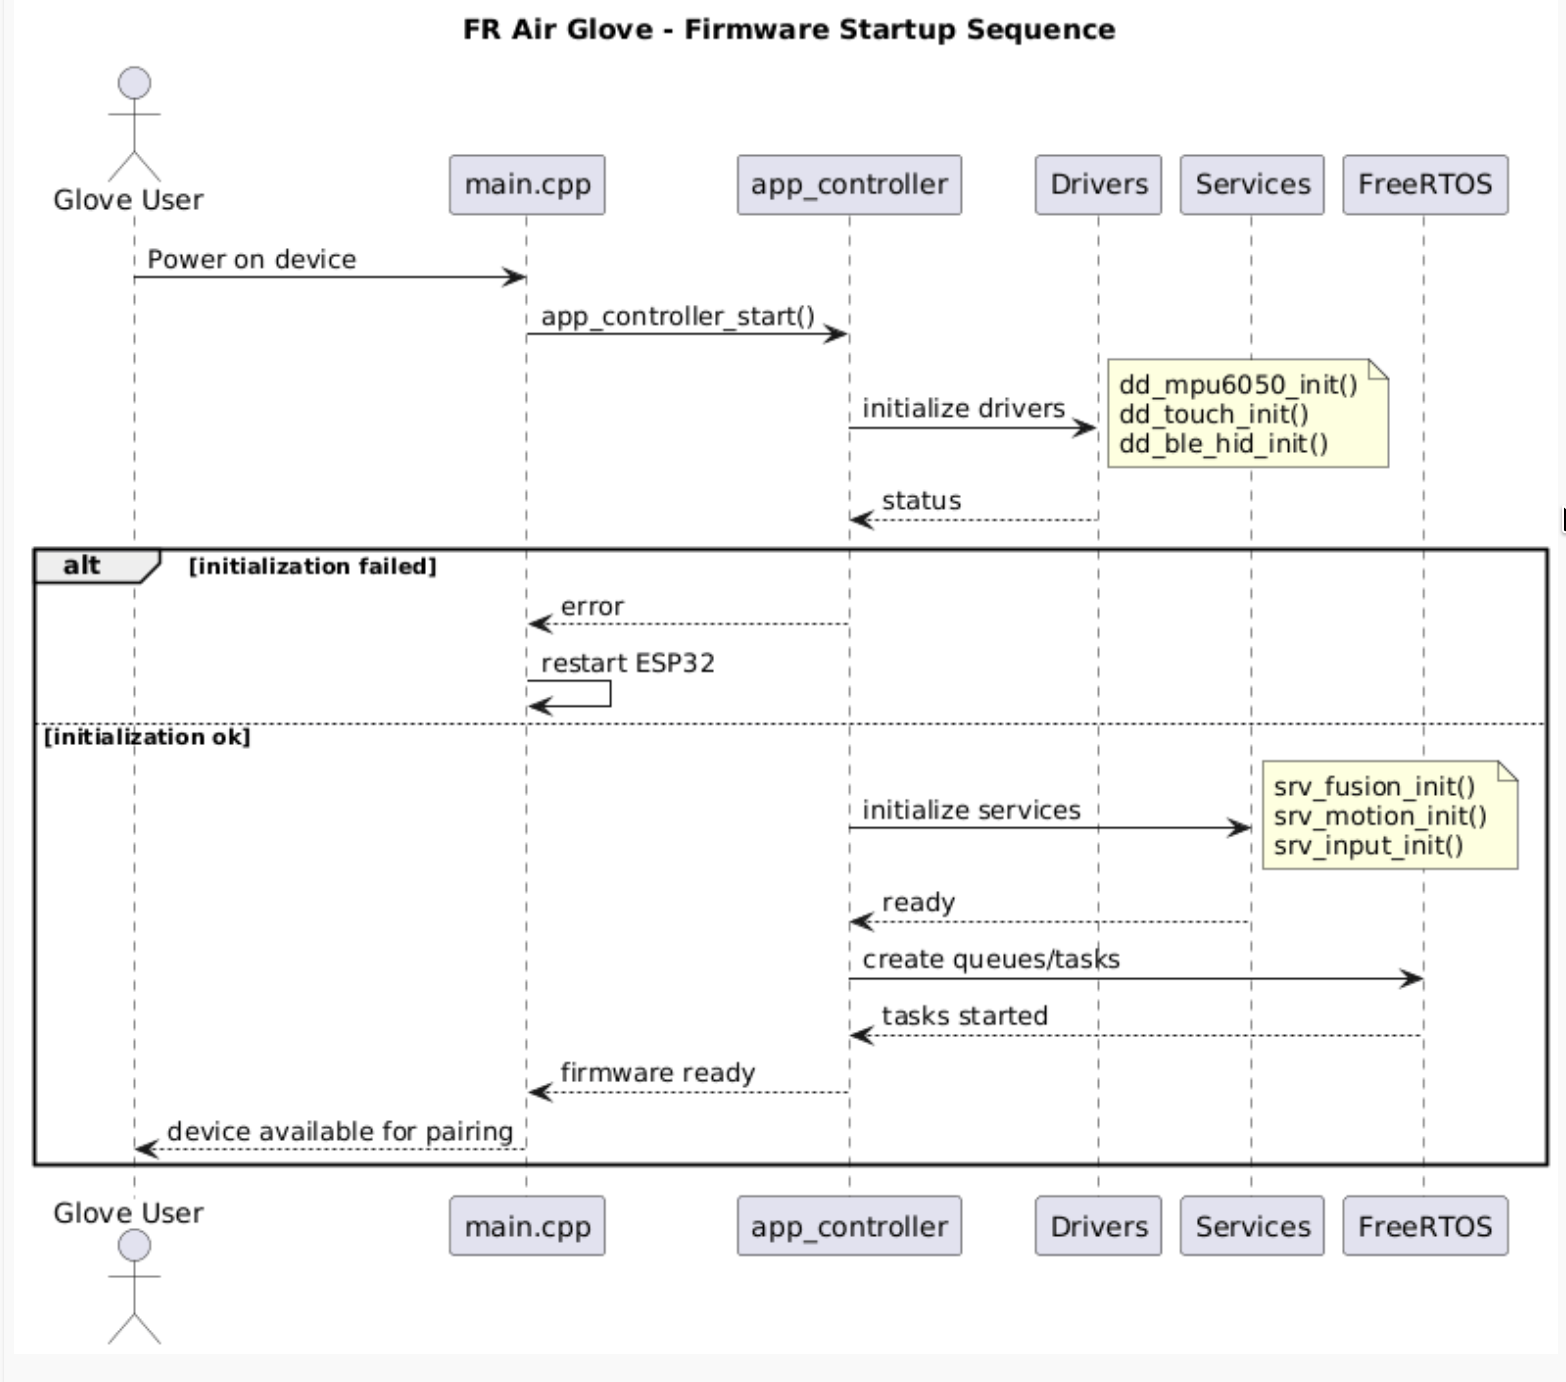
\includegraphics[width=0.5\textwidth]{img/s1.png}
    \caption{FR Air Glove Firmware Startup Sequence Diagram}
    \label{fig:fr-air-glove-sequence-startup}
\end{figure}

The firmware startup sequence diagram shows how the system components interact when the device is powered on. The glove user powers on the ESP32, which starts execution in \texttt{main.cpp}. The main file calls the application controller, and the controller initializes the internal system.

The controller first initializes the hardware drivers. These include the IMU driver, touch driver, and BLE HID driver. The drivers return their status to the controller. If initialization fails, the controller returns an error and the system restarts. If initialization succeeds, the controller continues by initializing services and creating FreeRTOS queues and tasks.

The final result of a successful startup is that the firmware becomes ready and the device becomes available for BLE pairing. This is a realistic representation because the user does not directly receive software messages; instead, the user observes that the device is available through its BLE behavior.

Code support examples:
\begin{itemize}
    \item \texttt{main.cpp} calls \texttt{app\_controller\_start()}.
    \item Driver initialization includes \texttt{dd\_mpu6050\_init()}, \texttt{dd\_touch\_init()}, and \texttt{dd\_ble\_hid\_init()}.
    \item Service initialization includes \texttt{srv\_fusion\_init()}, \texttt{srv\_motion\_init()}, and \texttt{srv\_input\_init()}.
    \item FreeRTOS queues and tasks are created during controller startup.
\end{itemize}

\subsubsection{Motion to Cursor Sequence}

\begin{figure}[H]
    \centering
    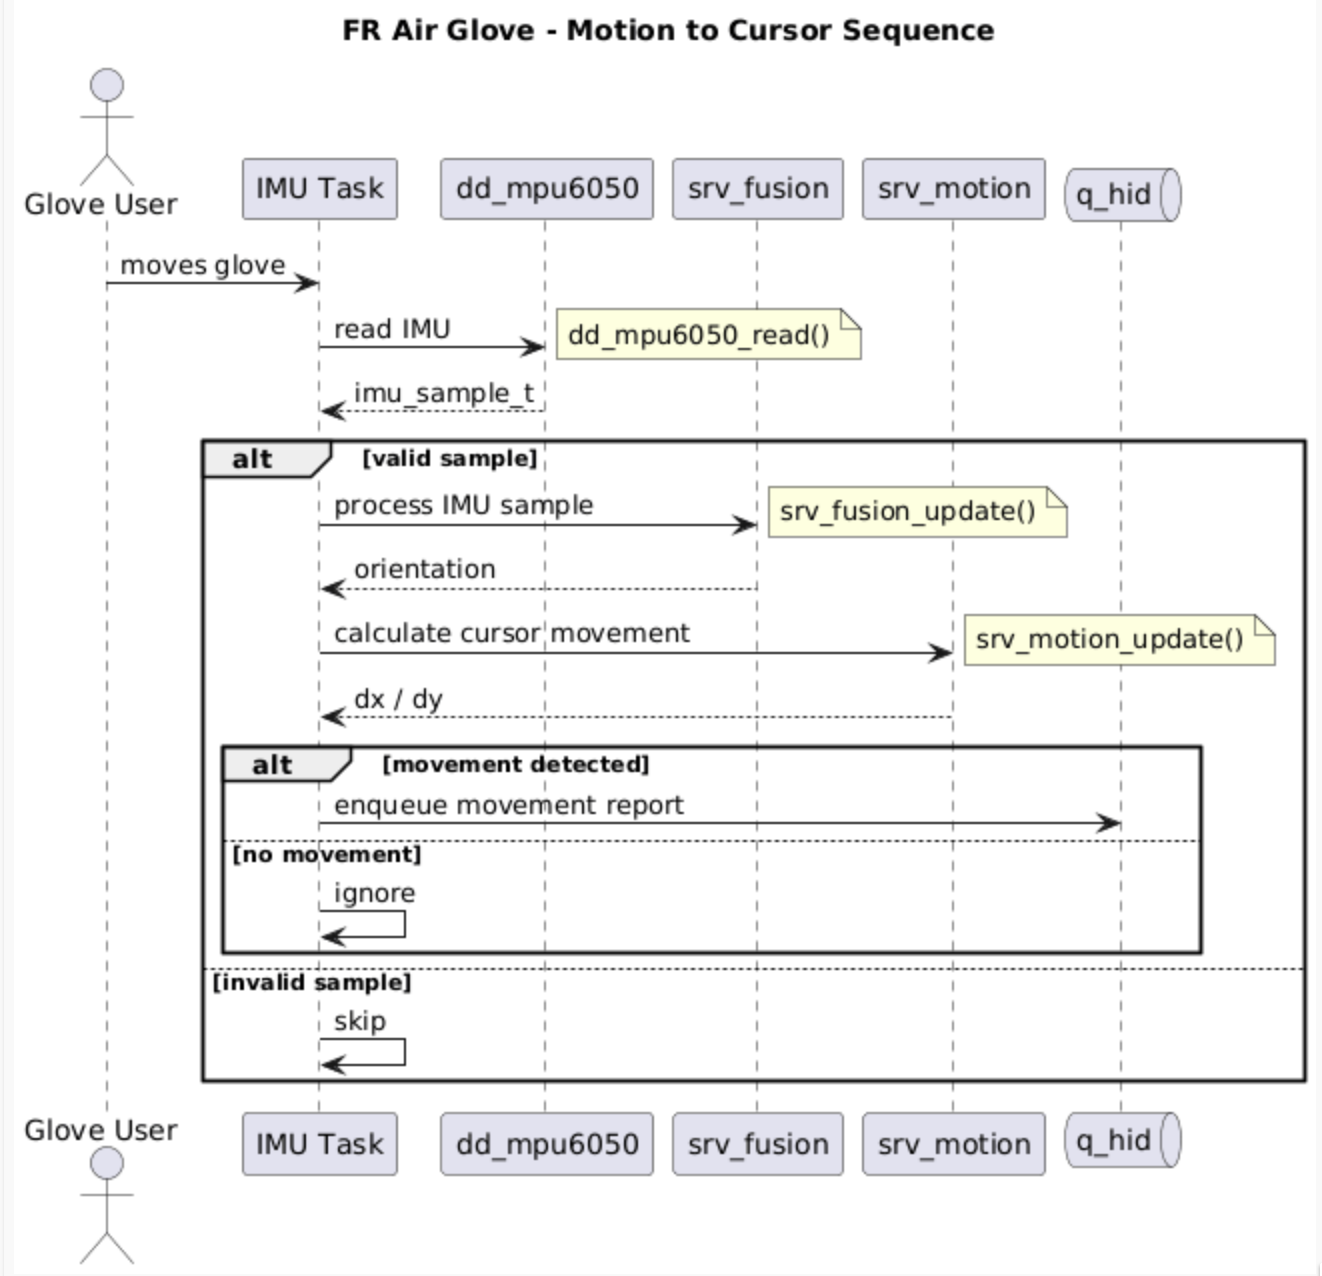
\includegraphics[width=0.5\textwidth]{img/s2.png}
    \caption{FR Air Glove Motion to Cursor Sequence Diagram}
    \label{fig:fr-air-glove-sequence-motion}
\end{figure}

The motion to cursor sequence diagram shows how the user's physical hand movement is transformed into mouse cursor movement. The glove user moves the device, and the IMU task reads motion data using the MPU6050 driver. The driver returns an IMU sample to the task.

If the sample is valid, the data is processed by the fusion service, which estimates the orientation of the glove. This orientation is then passed to the motion service, which calculates cursor movement values such as \texttt{dx} and \texttt{dy}. If movement is detected, a movement report is placed into the HID queue. If no movement is detected, the sample is ignored.

This sequence diagram is useful because it shows that cursor movement is not generated directly from raw sensor values. Instead, the firmware uses a processing chain: sensor reading, orientation estimation, movement calculation, and HID report creation.

Code support examples:
\begin{itemize}
    \item The IMU task reads sensor data using \texttt{dd\_mpu6050\_read()}.
    \item Orientation is estimated using \texttt{srv\_fusion\_update()}.
    \item Cursor movement is calculated using \texttt{srv\_motion\_update()}.
    \item Movement output is sent to the HID queue as a mouse movement report.
\end{itemize}

\subsubsection{Touch to Button Sequence}

\begin{figure}[H]
    \centering
    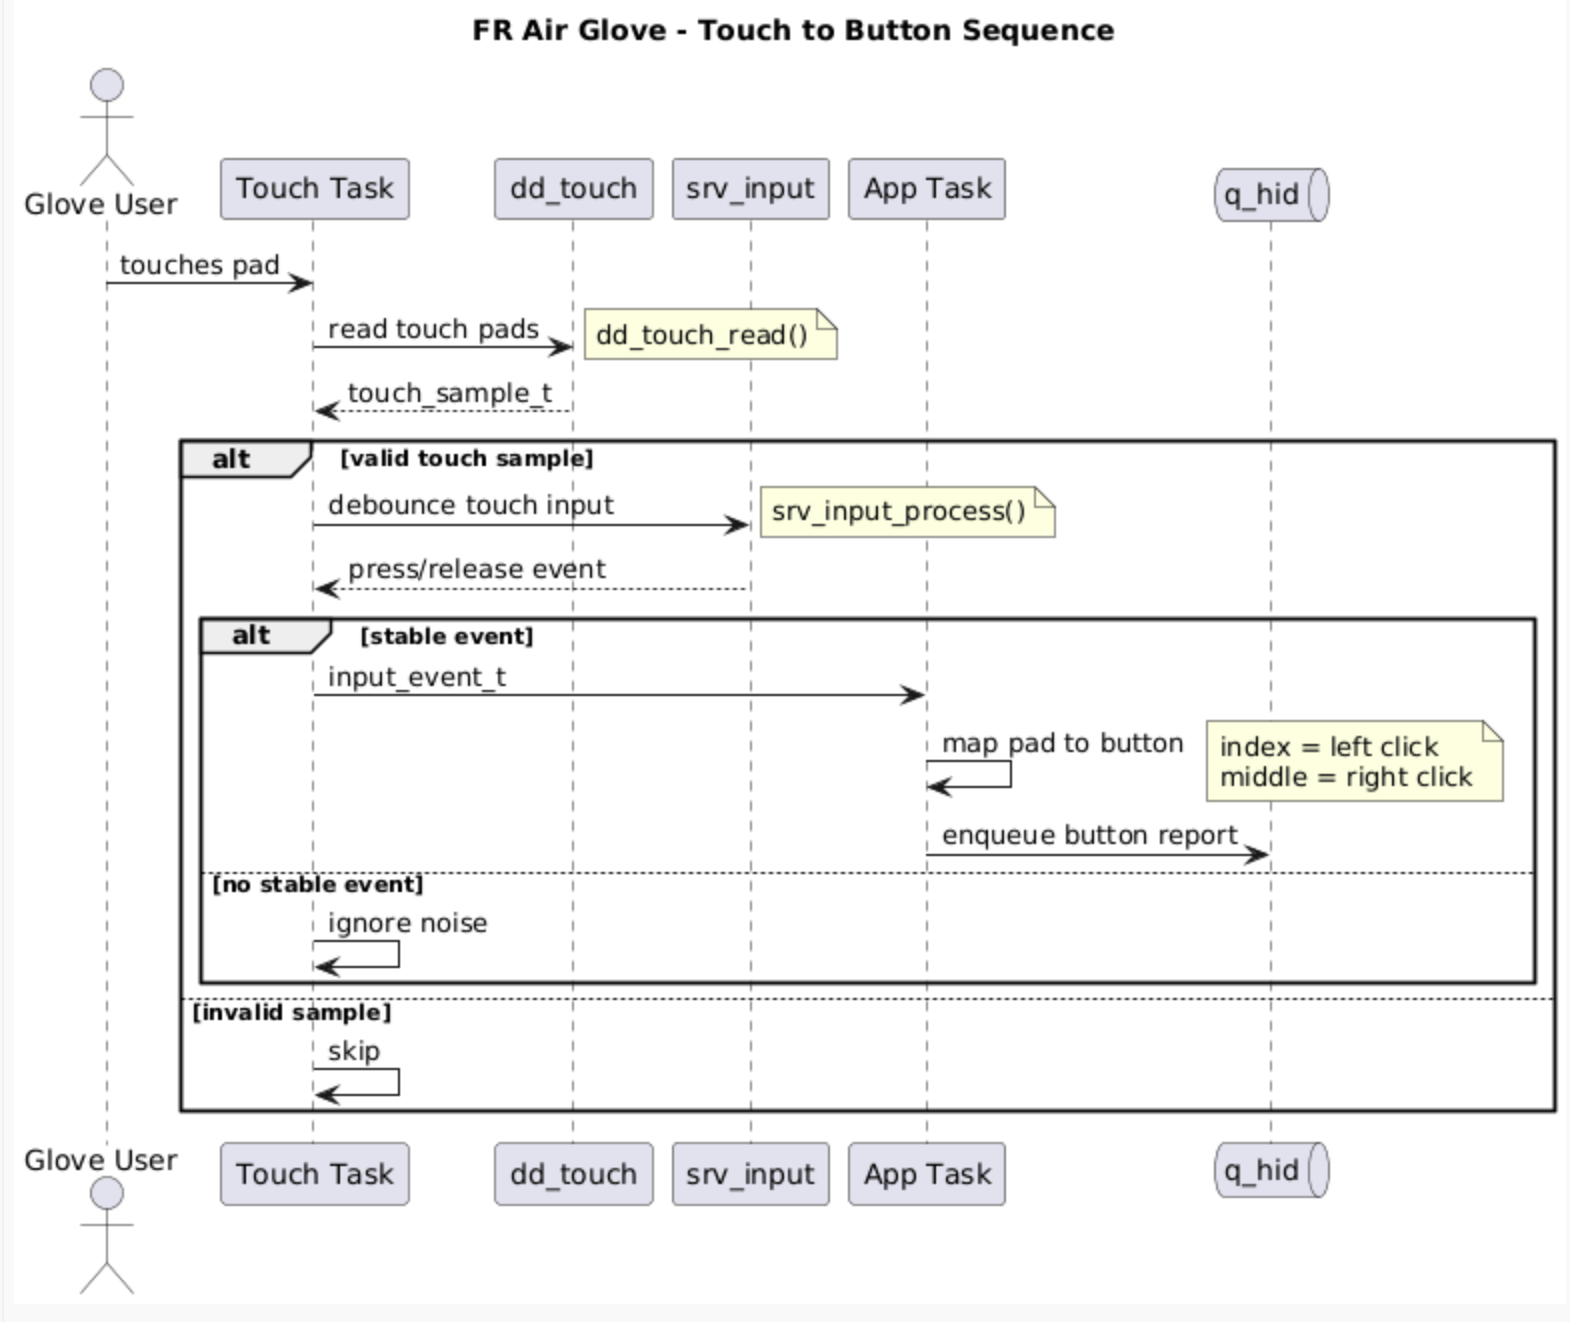
\includegraphics[width=0.5\textwidth]{img/s3.png}
    \caption{FR Air Glove Touch to Button Sequence Diagram}
    \label{fig:fr-air-glove-sequence-touch}
\end{figure}

The touch to button sequence diagram explains how a touch action becomes a mouse button report. The glove user touches one of the capacitive pads, and the touch task reads the pad values through the touch driver. The driver returns a touch sample to the task.

If the sample is valid, the input service processes it and checks whether a stable press or release event exists. This prevents unstable readings from becoming false button clicks. When a stable event is detected, the application task maps the pad to a mouse button. The index pad is mapped to the left click, while the middle pad is mapped to the right click. After mapping, the application task sends a button report to the HID queue.

This sequence diagram is useful because it clearly separates raw touch acquisition from input validation and button mapping. It also shows why the input service is needed before producing HID output.

Code support examples:
\begin{itemize}
    \item Capacitive touch values are read by \texttt{dd\_touch\_read()}.
    \item Touch validation and debounce are handled by \texttt{srv\_input\_process()}.
    \item Stable events are represented as press or release events.
    \item Button reports are sent to the HID queue after pad-to-button mapping.
\end{itemize}

\subsubsection{BLE HID Transmission Sequence}

\begin{figure}[H]
    \centering
    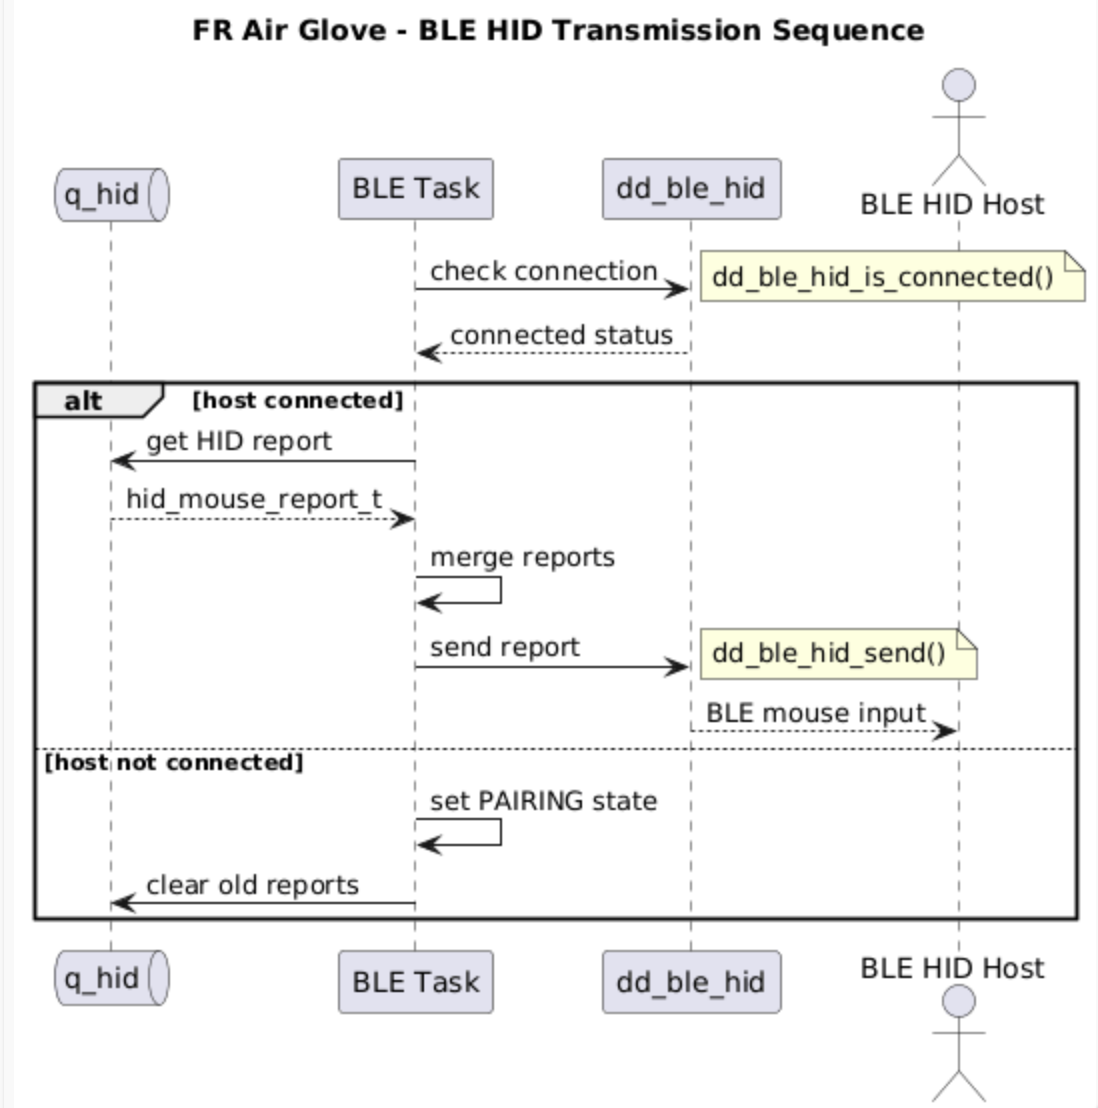
\includegraphics[width=0.5\textwidth]{img/s4.png}
    \caption{FR Air Glove BLE HID Transmission Sequence Diagram}
    \label{fig:fr-air-glove-sequence-ble}
\end{figure}

The BLE HID transmission sequence diagram describes how prepared HID reports are delivered to the external host device. The BLE task first checks the connection state through the BLE HID driver. The driver returns whether a host is connected or not.

If a host is connected, the BLE task reads a HID report from the HID queue. Before sending, it may merge pending reports to reduce unnecessary transmissions and preserve the latest button state. The final report is then sent through the BLE HID driver, and the BLE HID host receives it as mouse input.

If no host is connected, the firmware switches to pairing state and clears old HID reports. This prevents old movement or click data from being sent after a later reconnection.

This sequence diagram is useful because it shows that BLE transmission is isolated in a specific task and driver. Other modules only prepare reports; the BLE task decides when those reports can actually be sent.

Code support examples:
\begin{itemize}
    \item BLE connection is checked using \texttt{dd\_ble\_hid\_is\_connected()}.
    \item HID reports are taken from \texttt{q\_hid}.
    \item Report merging is handled inside the BLE task before sending.
    \item The final report is sent using \texttt{dd\_ble\_hid\_send()}.
\end{itemize}



